%===============================================================================
% Autoři: Michal Bidlo, Bohuslav Křena, Jaroslav Dytrych, Petr Veigend a Adam Herout 2018

\chapter{Úvod}
Bežný človek musí dennodenne riešiť rôzne typy úloh. Niektoré sú jednoduchšie, ako napríklad vyniesť odpadky, niektoré naopak zložitejšie, napríklad z pracovného prostredia. Cieľom každého z nás by malo byť efektívne riešenie týchto úloh. Informačné systémy riešia úlohy pomocou vopred definovaných postupov. Je rovnako dôležité aby aj tieto postupy boli dobre optimalizované. 

Dynamické programovanie (skrátene DP) \footnote{\textbf{DP} je často používaná skratka pre \textbf{D}ynamické \textbf{P}rogramovanie. Bude používaná aj v ďalším kapitolách tejto práce.} je optimalizačná metóda, ktorá môže podstatne zrýchliť výpočet určitého typu úloh. Princípom je ukladanie podvýsledkov, ktoré by inak boli vypočítavané znovu a znovu.

Moderná webová aplikácia, ktorá je výsledkom tejto práce vysvetľuje túto metódu na sérii príkladov. Používateľ aplikácie si môže sám zvoliť vstupné hodnoty a sledovať priebeh výpočtu. Okrem toho aplikácia vykresľuje aj grafy a tabuľky pre porovnanie štatistík pri jednoduchom riešení a pri využití dynamického programovania. Týmto sa líši od voľne dostupných webových prezentácií, ktoré síce poskytujú teóriu a riešenia veľkého počtu príkladov, ale neponúkajú grafické znázornenie princípu jednotlivých algoritmov.

Aplikácia má slúžiť hlavne ako podporný materiál pri výučbe. Využitie teda nájde najmä v akademickej sfére, ale zaujímavá môže byť pre každého kto sa aspoň trochu zaujíma o programovanie, algoritmy alebo aj matematické výpočty.

Následujúca kapitola tejto práce obsahuje nevyhnutnú teóriu k pochopenie princípov dynamického programovania, kedy je možné túto metódu použiť a aké výhody prináša. 

3. kapitola sa sústredí na návrh aplikácie. To zahŕňa výber technológií, návrh užívateľského rozhrania a štruktúry aplikácie. 

4. kapitola popisuje konkrétnu implementáciu. 5. kapitola sa zaoberá testovaním. Uvedené postrehy od študentov ale aj od bežných užívateľov, ktoré boli veľmi užitočné pre ladenie aplikácie.

Záverečná kapitola obsahuje zhrnutie výsledkov práce a ponúka možnosti na ďalšie vylepšenie a rozšírenie aplikácie.



\chapter{Dynamické programovanie}
\label{dynamickeProgramovanie}

V tejto kapitole sú preberané princípy optimalizačnej metódy -- dynamického programovania. Úvod kapitoly je zameraný na hlavné myšlienky tejto metódy, a teda rozdelenie úlohy na podproblémy a ukladanie dielčich výsledkov výpočtu. Z toho vyplývajú podmienky, ktoré musí naivné riešenie danej úlohy spĺňať aby sa miesto neho dalo použiť dynamické programovanie. Ďalej budú preberané konkrétne úlohy, ktoré sú súčasťou aplikácie. 

\section{Hlavné princípy dynamického programovania}

Dynamické programovanie je optimalizačná metóda, ktorá sa dá využiť pri riešení optimalizačných úloh \footnote{Optimalizačná úloha, je úloha, ktorá má viacero správnych riešení. Každé z týchto riešení má určitú hodnotu. Cieľom je nájsť extrém (najnižšiu alebo najvyššiu hodnotu). Riešení ktorých výsledkom je extrém môže byť viacero. Môže teda existovať viacero optimálnych riešení.\cite{IntroductionToAlg}}. Okrem oblasti informatiky sa s dynamickým programovaním môžme stretnúť napríklad aj v matematike. Názov tejto metódy môže byť preto trochu mätúci. Slovo \uv{programovanie} by malo poukazovať na \textbf{tabuľkovú metódu}.

Hlavným princípom metódy je dynamické ukladanie podvýsledkov do dátovej štruktúry (poľa alebo práve tabuľky), ktorých spojením sa dá určiť hodnota optimálneho riešenia, prípadne skonštruovať celé riešenie. Využíva rekurzívny rozklad problému na podproblémy \todo{labyrint algoritmu str.283}, podobne ako metóda \uv{Rozdeľuj a panuj}\todo{nieco k metode}. Jej výhoda ale spočíva práve v tom, že využíva opakovanie podproblémov a preto vedie často k oveľa rýchlejšiemu riešeniu.

Z týchto skutočností vyplývajú 2 podmienky nutné k tomu, aby daná úloha mohla byť riešená dynamickým programovaním:

\begin{enumerate}
    \item \textbf{Prekrývajúce sa podproblémy} \ref{prekryvPodProb}
    \item \textbf{Optimálna subštruktúra} \ref{optimalSubstrukt}
\end{enumerate}

\subsection{Prekrývanie podproblémov} \label{prekryvPodProb}
Ak sa pri riešení úlohy opakujú rovnaké podproblémy, je to prvým znamením, ktoré nabáda k využitiu dynamického programovania. Zistiť, či sa pri riešení úlohy vyskytujú podproblémy, ktorých výsledky sú vypočítavané viacnásobne sa dá zistiť jednoducho zakreslením \textbf{stromu rekurzie} \ref{stromRekurzie}.

\begin{figure} \label{stromRekurzie}
  \caption{Strom rekurzie graficky znázorňuje priebeh rekurzívneho riešenia úlohy. Pri uzloch vyznačených rovnakou farbou ide o rovnaké podproblémy, ktoré sú vypočítavané viacnásobne.}
  \centering
    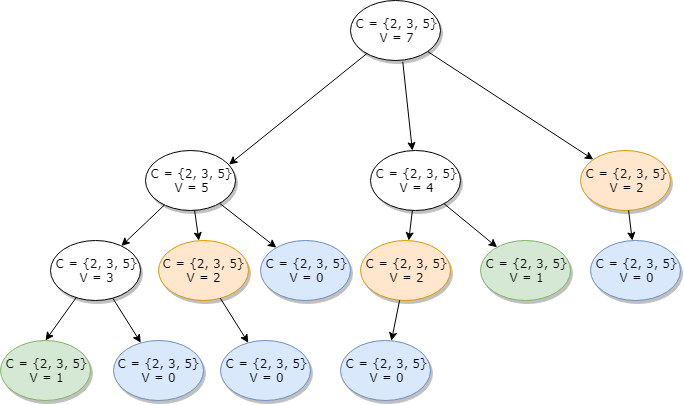
\includegraphics[width=0.8\textwidth]{obrazky-figures/coinsTree.png}
\end{figure}

Ak je zrejmé, že podproblémy sa neopakujú, použiť dynamické programovanie nemá zmysel. Práve naopak. Pri dynamickom programovaní by sa iba zvýšila \textbf{priestorová zložitosť} \todo{co je to} algoritmu z dôvodu vytvorenia dátovej štruktúry na ukladanie podvýsledkov. 

\subsection{Optimálna subštruktúra} \label{optimalSubstrukt}
Druhou vlastnosťou, ktorú musí optimalizačná úloha spĺňať sa nazýva \textbf{optimálna subštruktúra}. V prvom rade sa musí dať úloha rozdeliť na podproblémy. Každý z týchto podproblémov má vlastné optimálne riešenie. Ak sa spojením týchto čiastkových riešení dá dostať optimálne riešenie celej úlohy, dá sa konštatovať, že úloha má optimálnu subštruktúru. \cite{IntroductionToAlg}

\section{Vytvorenie algoritmu využívajúceho dynamické programovanie}

Vytvorenie efektívneho algoritmu postaveného na princípoch dynamického programovania zahŕňa obvykle 4 kroky:

\begin{enumerate}
    \item \textbf{Charakterizovanie štruktúry optimálneho riešenia úlohy} \ref{charakterStrukt}
    \item \textbf{Definovanie hodnoty optimálneho riešenia úlohy pomocou rekurzie} \ref{defOptRies}
    \item \textbf{Výpočet hodnoty optimálneho riešenia pomocou tabuľkovej metódy} \ref{vypocetHodnoty}
    \item \textbf{Zostavenie optimálneho riešenia s využitím vypočítaných hodnôt} \ref{zostavRies}
\end{enumerate}

Kroky 1.-3. je potrebné vykonať vždy. 4. krok je potrebný v prípade, ak je potrebné okrem hodnoty optimálneho riešenia zostaviť aj celé riešenie. Všetky kroky budú vysvetlené na nasledujúcom príklade, ktorý je aj súčasťou výslednej aplikácie: 

\begin{example}
%\textnormal{\textbf{Minimálny počet mincí na vytvorenie danej hodnoty}}
Majme neobmedzený počet mincí rôznych hodnôt $C=(c1, c2, c3, ..., cN)$ a hodnotu, ktorá má vzniknúť súčtom hodnôt mincí. Pre súčet musí byť využitý čo najmenší počet mincí. Ktoré mince budú použité a aký je ich počet?
\end{example}

\subsection{Charakterizovanie štruktúry optimálneho riešenia úlohy} \label{charakterStrukt}

V prvom kroku je potrebné danú optimalizačnú úlohu analyzovať. Dôležité je určiť si jednoduché vstupné hodnoty, aby sa dalo k optimálnemu riešeniu dostať stratégiou \uv{pokus--omyl}. Budú sa teda testovať kombinácie všetkých možných hodnôt, až nakoniec vypadne najoptimálnejšia kombinácia alebo aj viacero kombinácií s rovnakou výslednou hodnotou. Pri tomto naivnom zisťovaní výsledku sa dajú vyvodiť potrebné informácie, ktoré potvrdia alebo vyvrátia podmienky potrebné k tomu aby sa dal vytvoriť DP algoritmus.

\bigskip 

\noindent Určíme si vstupné hodnoty úlohy: 
\begin{itemize}
    \item Mince: 1, 2, 3, 5
    \item Hodnota: 8
\end{itemize}

Na prvý pohľad je jasné, že riešením je použiť 8 mincí s hodnotou 1, ale toto riešenie by nebolo optimálne. Skúsime teda použiť mincu s hodnotou 2. Aby sme v súčte dostali hodnotu 8, musíme pridať ďalšie 3 mince s hodnotou 2, prípadne použiť mincu s hodnotou 5 a pridať ešte mincu s hodnotou 1. Vypíšme si teda niektoré riešenia úlohy:

\begin{itemize}
    \item 2 + 2 + 2 + 2 = 8
    \item 2 + 2 + 3 + 1 = 8
    \item 2 + 3 + 3 = 8
    \item 3 + 2 + 2 + 1 = 8
    \item 5 + 2 + 1 = 8
    \item 5 + 3 = 8
\end{itemize}

Ak vyberieme mincu s hodnotou 2, musíme ďalej riešiť podproblém, kedy potrebujeme získať v súčet 6. Pridáme napríklad mincu s hodnotou 3. Ďalší podproblém bude získať súčet 3. Ten môžeme získať pridaním jednej mince s hodnotou 3 alebo mincí s hodnotami 2 a 1. Optimálne je vybrať minci s hodnotou 3. Takto nám vznikajú podproblémy, ktoré je možné riešiť nezávisle , a ktorých optimálnym riešením získame aj optimálne riešenie pôvodnej úlohy. Tým sme dokázali, že riešenie úlohy má \textbf{optimálnu subštruktúru}.

Pri tomto konkrétnom zadaní môže byť optimálne riešenie jasné. Je ním posledné riešenie, a teda súčet mincí s hodnotami 5 a 3. Minimálny počet mincí je teda 2. Problém by nastal pri zadaní viacerých typov mincí a vyššej hodnoty. Ďalším krokom je teda vytvorenie algoritmu. 

Pozn.: Okrem optimálneho riešenia si môžeme všimnúť, že niektoré podproblémy sú riešené viacnásobne, čo sa nám aj potvrdí po navrhnutí rekurzívneho algoritmu.

\subsection{Definovanie hodnoty optimálneho riešenia úlohy pomocou rekurzie} \label{defOptRies}

Po charakterizovaní štruktúry optimálneho riešenia vzhľadom na podproblémy nasleduje 2. krok. Ten spočíva v návrhu rekurzívneho algoritmu, využijeme teda metódu \uv{Zhora dole} \footnote{\textbf{Zhora dole} je metóda návrhu algoritmu. Princípom je postupné rozkladanie riešenia na jednoduchšie operácie až k elementárnym krokom.} k vytvoreniu formuly. Ako vzor poslúži opäť príklad s mincami. 

V prvom rade vezmeme do úvahy špecifický prípad, od ktorého sa odrazíme. Ak je zadaná hodnota rovná 0, aj počet mincí bude 0. Ak je hodnota väčšia ako 0, zoberieme postupne všetky mince, ktorých hodnota je menšia alebo rovná požadovanej hodnote. Od požadovanej hodnoty sa odpočíta hodnota mince a rekurzívne sa zavolá rovnaká metóda pre túto novú požadovanú hodnotu, pričom sa inkrementuje počet použitých mincí. Riešenie možno popísať formulou (kód v jazyku C je v prílohe):

$$
minMince(m[0..p - 1], h) = min
\left\{
\begin{array}{ll}
1 + minMince(m, h - m[i]) &\ \text{kde}\ 0 \leq i \leq p - 1\\
0 &\ \text{ak}\ h=0
\end{array}
\right.
$$

\begin{itemize}
    \item m - zadané mince
    \item p - počet mincí
    \item h - zadaná hodnota
\end{itemize}

Kód v jazyku C:



\subsection{Výpočet hodnoty optimálneho riešenia pomocou tabuľkovej metódy} \label{vypocetHodnoty}
\subsection{Zostavenie optimálneho riešenia s využitím vypočítaných hodnôt} \label{zostavRies}

\subsection{Rekonštrukcia optimálneho riešenia úlohy}

\section{Optimalizačné úlohy riešiteľné dynamickým programovaním}
\subsection{Minimálny počet mincí na vytvorenie danej hodnoty}
\subsection{Problém rezania tyče}
\subsection{Najdlhší spoločný podreťazec}
\subsection{Editačná vzdialenosť}
\subsection{Optimalizovaný binárny vyhľadávací strom}

\chapter{Návrh webovej aplikácie} 
\label{navrhAplikacie}
\section{Webové stránky so zameraním na dynamické programovanie - súčasný stav}
\section{Požiadavky kladené na novú webovú aplikáciu}
\section{Výber technológií pre vytvorenie modernej webovej aplikácie}
\subsection{React}
\subsection{Typescript}
\section{Návrh užívateľského rozhrania}
\subsection{Rozdelenie do kontajnerov}
\subsection{Teória}
\subsection{Demo}
\subsection{Grafy}

\chapter{Implementácia}
\label{implementacia}
\section{Štruktúra zdrojových textov}
\section{Zapúzdrenie do komponent}
\section{Hlavné časti aplikácie }
\subsection{Teória}
\todo{Zobrazenie zdrojových textov}
\subsection{Demo}
\todo{Vykresľovanie tabuľky}
\subsection{Grafy}
\todo{Vykresľovanie grafov}
\todo{Počítanie štatistik}

\chapter{Testovanie}
\label{testovanie}
\section{Testovací scenár}
\section{Testovanie s používateľmi}
\section{Vyhodnotenie testov}
\section{Úpravy aplikácie}

\chapter{Zaver}
\label{zaver}